\question (华中科技大学,2007年)若已知一个栈的入栈序列为1,2,3,4,其出栈序列为p1,p2,p3,p4,则p2,p4不可能是(
)
\par\twoch{2、4}{2、1}{\textcolor{red}{4、3}}{3、4}
\begin{solution}用排除法。A的操作序列为push,pop,push,pop,push,pop,push,pop。
B的操作序列为push,push,push,pop,pop,push,pop,pop。
D的操作序列为push,pop,push,psuh,pop,pop,push,pop。
只有C没有对应的操作序列,故选C。
\end{solution}
\question (武汉大学,2006年)设n个元素进栈序列是1,2,3,
,n,其输出序列是p1,p2, ,pn,若p1=3,则p2的值为( )
\par\twoch{一定是2}{一定是1}{\textcolor{red}{不可能是1}}{以上都不对}
\begin{solution}p1是3,即3出栈了,此时栈中剩下1,2,此时若出栈,就是2,不可能是1。但又因为后面还有进栈元素,因此也可能是其他元素。综上分析,可能是2,不可能是1,因此本题选C。
\end{solution}
\question 设栈S和队列Q的初始状态均为空,元素a,b,c,d,e,f,g依次进入栈S。若每个元素出栈后立即进入队列Q,且7个元素出队的顺序是b,d,c,f,e,a,g,则栈S的容量至少是(
~)
\par\twoch{1}{2}{\textcolor{red}{3}}{4}
\begin{solution}首先队列不改变进出序列,故本题等价于入栈顺序a,b,c,d,e,f,g。出栈顺序为b,d,c,f,e,a,g,求栈空间至少多大。栈操作的过程如下所示,可以看到,栈中最多有3个元素,即栈大小至少为3。
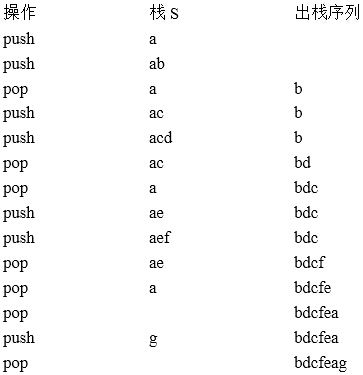
\includegraphics[width=3.78125in,height=3.90625in]{computerassets/13bba34f34f8765d413e9d53bfddf745.jpeg}
【总结】
栈和队列相关的题目并不难,只要根据入栈顺序和出栈顺序,还原栈操作过程,就能够得到正确的答案。
\end{solution}
\question 若元素a,b,c,d,e,f依次进栈,允许进栈、退栈操作交替进行,但不允许连续三次进行退栈操作,则不可能得到的出栈序列是(
)
\par\twoch{d,c,e,b,f,a}{c,b,d,a,e,f}{b,c,a,e,f,d}{\textcolor{red}{a,f,e,d,c,b}}
\begin{solution}A选项:入栈顺序为:a,b,c,d,e,f。出栈顺序为:d,c,e,b,f,a。
B选项:入栈顺序为:a,b,c,d,e,f。出栈顺序为:c,b,d,a,e,f。
C选项:入栈顺序为:a,b,c,d,e,f。出栈顺序为:b,c,a,e,f,d。
D选项:入栈顺序为:a,b,c,d,e,f。出栈顺序为:a,f,e,d,c,b。按照题设要求,选项D所给序列即为不可能得到的出栈顺序,因为其最后是连续的5个pop(出栈)操作。
\end{solution}
\question 元素a,b,c,d,e依次进入初始为空的栈中,若元素进栈后可停留、可出栈,直到所有的元素都出栈,则在所有可能的出栈序列中,以元素d开头的序列个数是(
)
\par\twoch{3}{\textcolor{red}{4}}{5}{6}
\begin{solution}若要保证出栈序列以d开头,则前3个元素必连续进栈,中间不能出现出栈的情况,然后d出栈,此时栈内元素由底到顶为,a,b,c,栈外元素为e,出栈序列中元素为d。
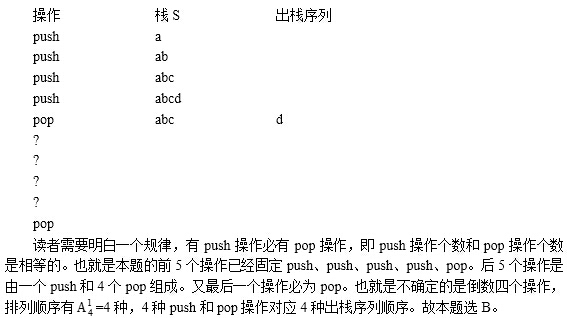
\includegraphics[width=5.90625in,height=3.31250in]{computerassets/e6ce6cda40e4109f129b7eaf9d62c8e2.jpeg}
【总结】
除了根据push和pop操作来确定,本题也可以通过序列的排列顺序来判定,首先a,b,c,d这4个元素在栈内的顺序已定,由栈的先进后出原则,其在出栈序列中的相对位置必为\ldots{}d\ldots{}c\ldots{}b\ldots{}a\ldots{};又因为d的位置已定,所以出栈待定序列必为d\ldots{}c\ldots{}b\ldots{}a\ldots{}。显然在栈外的e可以在任何时候出栈入栈,即可以出现在以上待定序列中任何一个省略号的位置,即出栈序列有4种可能,故选B。
\end{solution}
\question (浙江大学,2005年)当字符序列t3\_依次入栈,输出长度为3的,且可用做C语言标识符的序列有(
)
\par\twoch{4个}{5个}{\textcolor{red}{3个}}{6个}
\begin{solution}此题当然可以采用枚举法,先找出合法的出栈序列,然后找出符合C语言标识符命名规则的那些序列,但是这样比较麻烦;因为是选择题,我们利用栈的数学性质,我们知道栈的出栈序列的个数满足Cantalan函数,即3个字符的出栈序列的个数一共有5个,另外出去以数字开头的3t\_和3\_t不能作为C语言的标识符外,一共可用的标识符序列共有3个
\end{solution}
\question (重庆大学,2004年)设有一足够大的栈,入栈序列为x,y,z,u,v,下列哪一个出栈序列是不可能的序列(
)
\par\twoch{x,y,z,u,v}{y,x,z,u,v}{\textcolor{red}{z,x,y,u,v}}{v,u,z,y,x}
\begin{solution}由于栈的先进后出规律,在给定的输入序列后,有些输出序列是不可能出现的,比如z,x,y,u,v。因为第一个输出是z,这时x,y一定是已进入栈了。这时栈里面依次是x和y,只可能是y先出,x后出
\end{solution}
\question (北京航空航天大学,2004年)若某堆栈的输入序列为1,2,3\ldots{}\ldots{},n,输出序列的第一个元素为n,则第i个输出元素为(
)
\par\twoch{i}{n-i}{\textcolor{red}{n-i+1}}{哪个元素无所谓}
\begin{solution}每次栈输出后,栈顶元素依次减1,所以第i个元素输出后,栈顶元素为n-i,而输出的元素为n-i+1
\end{solution}
\question (武汉大学,2005年)设栈S和队列Q的初始状态为空,6个元素入栈的顺序为:a1,a2,a3,a4,a5,a6。一个元素出栈后立即进入队列Q,若6个元素出队的顺序是:a2,a4,a3,a6,a5,a1,则栈S的容量至少应该是(
)
\par\twoch{2}{\textcolor{red}{3}}{4}{6}
\begin{solution}考察栈和队列的特点。栈的特点是后进先出,而队列是先进先出,当a2出栈时,栈中还有a1,当a4出栈时,栈中有元素a1,a3,即此时栈的容量至少为3,当a6出栈时,栈中还有元素a5和a1,故栈S的容量至少为3
\end{solution}
\question (南京林业大学,2005年)设有一个空栈,栈顶指针为1000H(十六进制,下同,且设每个入栈元素需要1个单位存储空间),现有输入序列1,2,3,4,5,经过push,push,pop,push,pop,push,pop,push后,栈顶指针是(
)
\par\twoch{\textcolor{red}{1002H}}{1003H}{1004H}{1005H}
\begin{solution}栈顶指针的位置只与执行的操作有关,和插入的元素的具体值无关,一共经历了5次压栈,三次出栈,则栈中增加了两个元素,故栈顶指针为1002H
\end{solution}
\question 下列关于栈的说法中,正确的是( )。
Ⅰ.若进栈顺序为a、b、c,则通过出栈操作可能得到5个a、b、c的不同排列
Ⅱ.链式栈的栈顶指针一定指向栈的链尾
Ⅲ.两个栈共享一个向量空间的好处是减少了存取时间
\par\twoch{\textcolor{red}{仅Ⅰ}}{仅Ⅰ、Ⅱ}{仅Ⅱ}{仅Ⅱ、Ⅲ}
\begin{solution}Ⅰ:该选项旨在让考生知道一个公式。对于n个不同元素进栈,出栈序列的个数满足Catalan函数可以马上得出,当n=3时,出栈序列个数为5故Ⅰ正确。
Ⅱ:链式栈一般采用单链表,栈顶指针即为链头指针。进栈和出栈均在链头进行,每次都要修改栈顶指针,链空即栈空(top==NULL),故Ⅱ错误。
Ⅲ:由于栈中数据的操作只有入栈和出栈,且时间复杂度均为O(1),因此并没有减少存取时间,故Ⅲ错误。
\end{solution}
